\documentclass[a4paper,11pt]{report}
\usepackage{chuan_math_gkt}
\usetikzlibrary{angles,quotes,intersections,patterns,decorations.pathreplacing}
\chuanexamsetup

\begin{document}
\examfontsize

\examsecret{绝密$\bigstar$启用前}

\examtitle{2020年普通高等学校招生全国统一考试（新高考I卷）}{数\quad 学}

\noticetitle
\begin{examnotice}
\item 答卷前，考生务必将自己的姓名、准考证号填写在答题卡上. 
\item 回答选择题时，选出每小题的答案后，用铅笔把答题卡上对应题目的答案标号涂黑. 如需改动，用橡皮擦干净后，再选涂其他答案标号. 回答非选择题时，将答案写在答题卡上. 写在本试卷上无效. 
\item 考试结束后，将本试卷和答题卡一并交回. 
\end{examnotice}

\examsection{一、选择题：本题共8小题，每小题5分，共40分. 在每小题给出的四个选项中，只有一项是符合题目要求的.}
\begin{examquestions}

\item 设集合 $A=\{x\mid 1\leq x\leq3\}$，$B=\{x\mid 2<x<4\}$，则 $A\cup B=$
\fourchoices
{$\{x\mid 2<x\leq3\}$}
{$\{x\mid 2\leq x\leq3\}$}
{$\{x\mid 1\leq x<4\}$}
{$\{x\mid 1<x<4\}$}

\item $\dfrac{2-\mathrm{i}}{1+2\mathrm{i}}=$
\fourchoices{$1$}{$-1$}{$\mathrm{i}$}{$-\mathrm{i}$}

\item $6$ 名同学到甲、乙、丙三个场馆做志愿者，每名同学只去 $1$ 个场馆，甲场馆安排 $1$ 名，乙场馆安排 $2$ 名，丙场馆安排 $3$ 名，则不同的安排方法共有
\fourchoices{$120$ 种}{$90$ 种}{$60$ 种}{$30$ 种}

\item 
\noindent\begin{minipage}[t]{0.63\linewidth}
日晷是中国古代用来测定时间的仪器，利用与晷面垂直的晷针投射到晷面的影子来测定时间. 把地球看成一个球（球心记为 $O$），地球上一点 $A$ 的纬度是指 $OA$ 与地球赤道所在平面所成角，点 $A$ 处的水平面是指过点 $A$ 且与 $OA$ 垂直的平面. 在点 $A$ 处放置一个日晷，若晷面与赤道所在平面平行，点 $A$ 处的纬度为北纬 $40^\circ$，则晷针与点 $A$ 处的水平面所成角为
\end{minipage}\hfill
\begin{minipage}[t]{0.32\linewidth}
\vspace{1em}
\centering
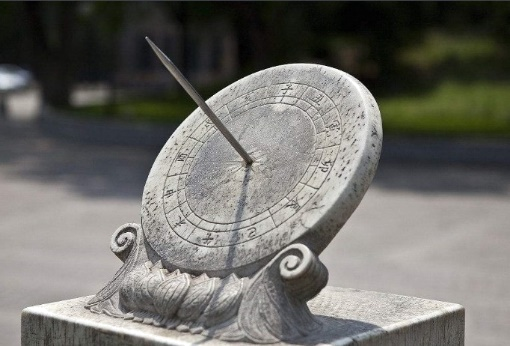
\includegraphics[width=4.2cm]{figures/2020_xgk1_image3.png}
\end{minipage}

\fourchoices{$20^\circ$}{$40^\circ$}{$50^\circ$}{$90^\circ$}

\item 某中学的学生积极参加体育锻炼，其中有 $96\%$ 的学生喜欢足球或游泳，$60\%$ 的学生喜欢足球，$82\%$ 的学生喜欢游泳，则该中学既喜欢足球又喜欢游泳的学生数占该校学生总数的比例是
\fourchoices{$62\%$}{$56\%$}{$46\%$}{$42\%$}

\item 基本再生数 $R_0$ 与世代间隔 $T$ 是新冠肺炎的流行病学基本参数. 基本再生数指一个感染者传染的平均人数，世代间隔指相邻两代间传染所需的平均时间. 在新冠肺炎疫情初始阶段，可以用指数模型 $I(t)=e^{rt}$ 描述累计感染病例数 $I(t)$ 随时间 $t$（单位：天）的变化规律，指数增长率 $r$ 与 $R_0,T$ 近似满足 $R_0=1+rT$. 有学者基于已有数据估计出 $R_0=3.28$，$T=6$. 据此，在新冠肺炎疫情初始阶段，累计感染病例数增加 $1$ 倍需要的时间约为（$\ln2\approx0.69$）
\fourchoices{$1.2$ 天}{$1.8$ 天}{$2.5$ 天}{$3.5$ 天}
\vspace{-0.3em}
\item 已知 $P$ 是边长为 $2$ 的正六边形 $ABCDEF$ 内的一点，则 $\vec{AP}\cdot\vec{AB}$ 的取值范围是
\fourchoices{$(-2,6)$}{$(-6,2)$}{$(-2,4)$}{$(-4,6)$}
\vspace{-0.3em}

\item 若定义在 $\mathbb R$ 的奇函数 $f(x)$ 在 $(-\infty,0)$ 单调递减，且 $f(2)=0$，则满足 $xf(x-1)\geq0$ 的 $x$ 的取值范围是
\fourchoices
{$[-1,1]\cup[3,+\infty)$}
{$[-3,-1]\cup[0,1]$}
{$[-1,0]\cup[1,+\infty)$}
{$[-1,0]\cup[1,3]$}

\end{examquestions}
\vspace{-1.2em}
\examsection{二、选择题：本题共4小题，每小题5分，共20分. 在每小题给出的选项中，有多项符合题目要求. 全部选对的得5分，部分选对的得2分，有选错的得0分.}
\begin{examquestions}[start=9]

\item 已知曲线 $C:mx^2+ny^2=1$.
\onechoices
{若 $m>n>0$，则 $C$ 是椭圆，其焦点在 $y$ 轴上}
{若 $m=n>0$，则 $C$ 是圆，其半径为 $\sqrt n$}
{若 $mn<0$，则 $C$ 是双曲线，其渐近线方程为 $y=\pm\sqrt{-\dfrac{m}{n}}x$}
{若 $m=0$，$n>0$，则 $C$ 是两条直线}

\item 
\noindent\begin{minipage}[t]{0.7\linewidth}
下图是函数 $y=\sin(\omega x+\varphi)$ 的部分图像，则 $\sin(\omega x+\varphi)=$

\twochoices
{\tallchoice{$\sin\left(x+\dfrac{\pi}{3}\right)$}}
{\tallchoice{$\sin\left(\dfrac{\pi}{3}-2x\right)$}}
{\tallchoice{$\cos\left(2x+\dfrac{\pi}{6}\right)$}}
{\tallchoice{$\cos\left(\dfrac{5\pi}{6}-2x\right)$}}
\end{minipage}\hfill
\begin{minipage}[t]{0.24\linewidth}
\vspace{-2.4em}
\centering
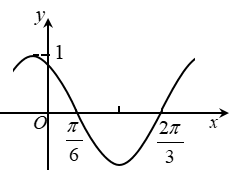
\includegraphics[width=4.5cm]{figures/2020_xgk1_image20.png}
\end{minipage}
\vspace{-2em}

\item 已知 $a>0$，$b>0$，且 $a+b=1$，则
\twochoices
{{$a^2+b^2\geq\dfrac12$}}
{{$2^{a-b}>\dfrac12$}}
{{$\log_2a+\log_2b\geq-2$}}
{{$\sqrt a+\sqrt b\leq\sqrt2$}}

\item 信息熵是信息论中的一个重要概念. 设随机变量 $X$ 所有可能的取值为 $1,2,\cdots,n$，且 $P(X=i)=p_i>0(i=1,2,\cdots,n)$，$\sum_{i=1}^{n}p_i=1$，定义 $X$ 的信息熵 $H(X)=-\sum_{i=1}^{n}p_i\log_2p_i$.
\onechoices
{若 $n=1$，则 $H(X)=0$}
{若 $n=2$，则 $H(X)$ 随着 $p_1$ 的增大而增大}
{若 $p_i=\dfrac1n(i=1,2,\cdots,n)$，则 $H(X)$ 随着 $n$ 的增大而增大}
{若 $n=2m$，随机变量 $Y$ 所有可能的取值为 $1,2,\cdots,m$，且 $P(Y=j)=p_j+p_{2m+1-j}(j=1,2,\cdots,m)$，则 $H(X)\leq H(Y)$}

\end{examquestions}

\examsection{三、填空题：本题共4小题，每小题5分，共20分.}
\begin{examquestions}[start=13]

\item 斜率为 $\sqrt3$ 的直线过抛物线 $C:y^2=4x$ 的焦点，且与 $C$ 交于 $A,B$ 两点，则 $|AB|=$ \blank.

\item 将数列 $\{2n-1\}$ 与 $\{3n-2\}$ 的公共项从小到大排列得到数列 $\{a_n\}$，则 $\{a_n\}$ 的前 $n$ 项和为 \blank.

\item 
\noindent\begin{minipage}[t]{0.63\linewidth}
某中学开展劳动实习，学生加工制作零件，零件的截面如图所示. $O$ 为圆孔及轮廓圆弧 $AB$ 所在圆的圆心，$A$ 是圆弧 $AB$ 与直线 $AG$ 的切点，$B$ 是圆弧 $AB$ 与直线 $BC$ 的切点，四边形 $DEFG$ 为矩形，$BC\perp DG$，垂足为 $C$，$\tan\angle ODC=\dfrac35$，$BH\parallel DG$，$EF=12\,\mathrm{cm}$，$DE=2\,\mathrm{cm}$，$A$ 到直线 $DE$ 和 $EF$ 的距离均为 $7\,\mathrm{cm}$，圆孔半径为 $1\,\mathrm{cm}$，则图中阴影部分的面积为 \blank $\mathrm{cm}^2$.
\end{minipage}\hfill
\begin{minipage}[t]{0.32\linewidth}
\vspace{1em}
\centering
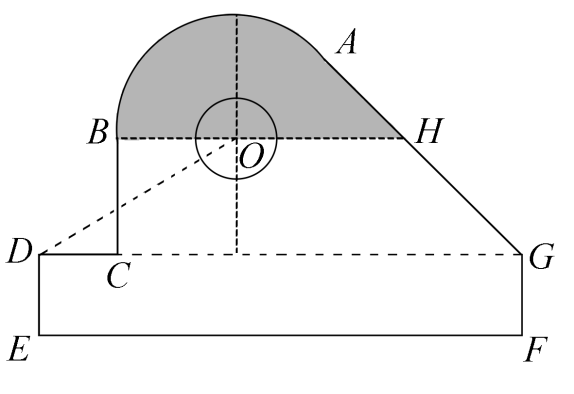
\includegraphics[width=4.8cm]{figures/2020_xgk1_image41.png}
\end{minipage}

\item 已知直四棱柱 $ABCD-A_1B_1C_1D_1$ 的棱长均为 $2$，$\angle BAD=60^\circ$. 以 $D_1$ 为球心，$\sqrt5$ 为半径的球面与侧面 $BCC_1B_1$ 的交线长为 \blank.

\end{examquestions}

\examsection{四、解答题：本题共6小题，共70分. 解答应写出文字说明、证明过程或演算步骤.}
\begin{examanswers}[start=17]

\item（10分）

在 \gktcircled{1} $ac=\sqrt3$，\gktcircled{2} $c\sin A=3$，\gktcircled{3} $c=\sqrt3b$ 这三个条件中任选一个，补充在下面问题中，若问题中的三角形存在，求 $c$ 的值；若问题中的三角形不存在，说明理由.

问题：是否存在 $\triangle ABC$，它的内角 $A,B,C$ 的对边分别为 $a,b,c$，且 $\sin A=\sqrt3\sin B$，$C=\dfrac{\pi}{6}$，\blank？

注：如果选择多个条件分别解答，按第一个解答计分.

\item（12分）

已知公比大于 $1$ 的等比数列 $\{a_n\}$ 满足 $a_2+a_4=20$，$a_3=8$.

\subq{（1）}{求 $\{a_n\}$ 的通项公式；}

\subq{（2）}{求 $a_1a_2-a_2a_3+\cdots+(-1)^{n-1}a_na_{n+1}$.}

\item（12分）

为加强环境保护，治理空气污染，环境监测部门对某市空气质量进行调研，随机抽查了 $100$ 天空气中的 $\mathrm{PM}_{2.5}$ 和 $\mathrm{SO}_2$ 浓度（单位：$\mu\mathrm{g}/\mathrm{m}^3$），得下表：

\begin{tightcenter}
{\renewcommand{\arraystretch}{0.9}
\begin{tabular}{|c|c|c|c|}
\hline
$\mathrm{SO}_2\backslash \mathrm{PM}_{2.5}$ & $[0,50]$ & $(50,150]$ & $(150,475]$\\ \hline
$[0,35]$ & $32$ & $18$ & $4$\\ \hline
$(35,75]$ & $6$ & $8$ & $12$\\ \hline
$(75,115]$ & $3$ & $7$ & $10$\\ \hline
\end{tabular}}
\end{tightcenter}

\subq{（1）}{估计事件“该市一天空气中 $\mathrm{PM}_{2.5}$ 浓度不超过 $75$，且 $\mathrm{SO}_2$ 浓度不超过 $150$”的概率；}

\subq{（2）}{根据所给数据，完成下面的 $2\times2$ 列联表：}

\begin{tightcenter}
{\renewcommand{\arraystretch}{0.9}
\begin{tabular}{|c|c|c|}
\hline
$\mathrm{SO}_2\backslash \mathrm{PM}_{2.5}$ & $[0,150]$ & $(150,475]$\\ \hline
$[0,75]$ &  & \\ \hline
$(75,115]$ &  & \\ \hline
\end{tabular}}
\end{tightcenter}

\subq{（3）}{根据（2）中的列联表，判断是否有 $99\%$ 的把握认为该市一天空气中 $\mathrm{PM}_{2.5}$ 浓度与 $\mathrm{SO}_2$ 浓度有关？附：$K^2=\dfrac{n(ad-bc)^2}{(a+b)(c+d)(a+c)(b+d)}$.}

\begin{tightcenter}
{\renewcommand{\arraystretch}{0.9}
\begin{tabular}{|c|c|c|c|}
\hline
$P(K^2\geq k)$ & $0.050$ & $0.010$ & $0.001$ \\ \hline
$k$ & $3.841$ & $6.635$ & $10.828$ \\ \hline
\end{tabular}}
\end{tightcenter}

\item（12分）

如图，四棱锥 $P-ABCD$ 的底面为正方形，$PD\perp$ 底面 $ABCD$. 设平面 $PAD$ 与平面 $PBC$ 的交线为 $l$.

\noindent\begin{minipage}[t]{0.62\linewidth}
\subq{（1）}{证明：$l\perp$ 平面 $PDC$；}

\subq{（2）}{已知 $PD=AD=1$，$Q$ 为 $l$ 上的点，求 $PB$ 与平面 $QCD$ 所成角的正弦值的最大值.}
\end{minipage}\hfill
\begin{minipage}[t]{0.25\linewidth}
\vspace{-1.9em}
\centering
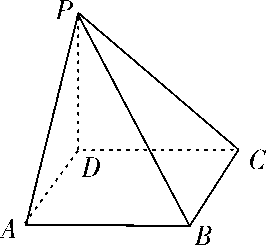
\includegraphics[width=4cm]{figures/2020_xgk1_image76.png}
\end{minipage}

\vspace{-3.2em}

\item（12分）

椭圆 $C:\dfrac{x^2}{a^2}+\dfrac{y^2}{b^2}=1(a>b>0)$ 过点 $M(2,3)$，点 $A$ 为左顶点，且 $AM$ 的斜率为 $\dfrac12$.

\subq{（1）}{求 $C$ 的方程；}

\subq{（2）}{点 $N$ 为椭圆上任意一点，求 $\triangle AMN$ 的面积的最大值.}

\item（12分）

已知函数 $f(x)=ae^{x-1}-\ln x+\ln a$.

\subq{（1）}{当 $a=e$ 时，求曲线 $y=f(x)$ 在点 $(1,f(1))$ 处的切线与两坐标轴围成的三角形的面积；}

\subq{（2）}{若 $f(x)\geq1$，求 $a$ 的取值范围.}

\end{examanswers}

\end{document}